% !TEX root = main.tex
\section{Nowa implementacja modułu AthenaMonitoring}
Głównym celem refaktoringu framworka, było oddzielenie kodu odpowiedzialnego za zarządzanie histogramami od kodu algorytmów. 
Dzięki takiemu rozgraniczeniu odpowiedzialności, twórcy algorytmów mogą skupić się na ich poprawnej implementacji i określeniu które wartości powinny znaleźć się na wykresach jako wynik. 
Natomiast to kiedy stworzyć histogram, jak go wypełnić i zapisać jest obsługiwane przez wspólny kod. 

Sercem nowego rozwiązania jest GenericMonitoringTool - nowe narzędzie w ramach frameworka Athena.
Zajmuje się on przygotowaniem histogramów i powiązaniem ich z kodem uruchamianych algorytmów. 
Działa on w oparciu o deklaracje.
Twórca algorytmu deklaruje zbiór wartości (obejmuje to skalary oraz tablice) jakie mogą być monitorowane w obrębie jego wykonania, oraz informuje GenericMonitoringTool kiedy są one gotowe do przekazania do histogramów.
Natomiast użytkownik takiego algorytmu, deklaruje jakie wykresy chciałby stworzyć i z użyciem których zmiennych. 
Następuje to w kroku konfiguracyjnym Athena Python, gdzie definiuje on typy histogramów, parametry binowania, zakresy wartości, opisy itd. 
Taki interfejs pozwala uniknąć rekompilacji kodu C++ za każdym razem, gdy użytkownik zmienia parametry wykresu. 

\begin{figure}[!ht]
\centering
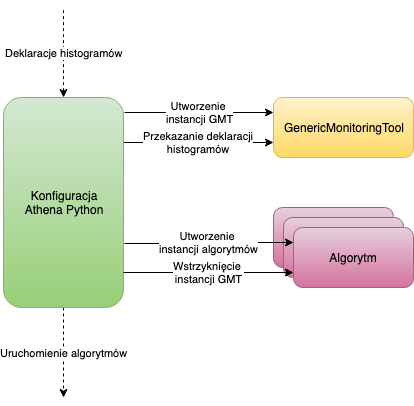
\includegraphics[width=0.75\textwidth]{img/algo_init.png}
\caption{
//TODO
}
\label{fig:athena:oldFlow}
\end{figure}

\begin{figure}[!ht]
\centering
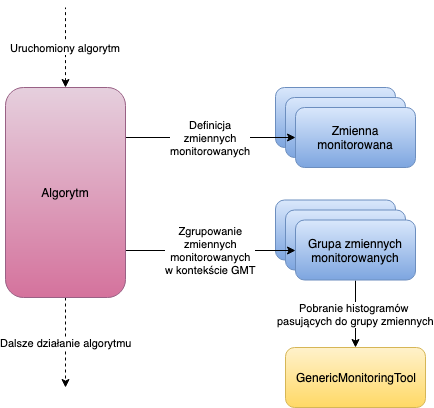
\includegraphics[width=0.75\textwidth]{img/algo_run.png}
\caption{
//TODO
}
\label{fig:athena:oldFlow}
\end{figure}

\subsection{Implementacja}

\begin{itemize}
\item GenericMonitoringTool
	\begin{itemize}
	\item public
	\item centralna klasa
	\item pomost pomiedzy konfiguracja python a kodem C++
	\item pozwala pobrac lumi block i run number
	\item pozwala pobrac histogram fillery pasujace do danej grupy zmiennych monitorowanych
	\item tworzy i trzyma histogram fillery dla kazdego zadeklarowanego histogramu
	\end{itemize}
	
\item HistogramDef
	\begin{itemize}
	\item public
	\item jest reprezentacja/definicją histogramu
	\item potrafi utworzyc siebie ze stringa podanego przez uzytkownika
	\item waliduje czy podane przez uzytkownika paramtery sa poprawne
	\item jesli nie to nie uda sie utworzyc 
	\end{itemize}
	
\item HistogramFactory
	\begin{itemize}
	\item stanowi polaczenie z frameworkiem ROOT
	\item to ona tworzy i konfiguruje histogramy w ramach THistSvc
	\item robi to na bazie HistogramDef
	\item obsluguje cacheowanie juz raz utworzonych histogramow - niezalecane
	\end{itemize}
	
\item HistogramException
	\begin{itemize}
	\item wyjatek rzucany gdy cos sie nie powiedzie przy tworzeniu/pobieraniu histogramu na podstawie histogramDef 
	\end{itemize}
	
\item IHistogramProvider
	\begin{itemize}
	\item public
	\item interfejs ktory pozwala pobierac histogramy ROOT 
	\end{itemize}
\item StaticHistogramProvider
	\begin{itemize}
	\item Implementacja IHistogramProvidera
	\item pobiera histogramy ROOT bezposrednio z HistogramFactory przy tworzeniu
	\item cacheuje je, nigdy sie nie zmienia
	\end{itemize}
\item LumiblockHistogramProvider
	\begin{itemize}
	\item Implementacja IHistogramProvidera
	\item pobiera histogramy ROOT z HistogramFactory na podstawie aktualnego lumi bloku
	\item za kazdym razem odwoluje sie na nowo do HF
	\item wazny jest parametr kLBNHistoryDepth podawany w definicji histogramu
	\item definiuje on na jak liczne grupy podzielone beda wyniki
	\item musi byc liczba dodatnia
	\end{itemize}
\item OfflineHistogramProvider
	\begin{itemize}
	\item przeznaczony dla uruchomien Offline
	\item pobiera histogramy ROOT z HistogramFactory na podstawie aktualnego lumi bloku, run number i konwencji histogramu 
	\end{itemize}
	
\item HistogramFillerFactory
	\begin{itemize}
	\item na podstawie HistogramDef decyduje jaka instancja HistogramProvidera ma zostac utworzona
	\item na podstawie HistogramDef decyduje jaka instancja HistogramFillera ma zostac utworzona
	\end{itemize}
\item HistogramFiller
	\begin{itemize}
	\item public
	\item oddziela swiat frameworka ROOT od frameworka athena
	\item klasa abstrakcyjna
	\item zapewnia interfejs do wypelniania histogramow ROOT
	\item pozwala wstrzyknac zmienne monitorowane ktore maja zostac uzyte przy wypelnianiu
	\item przechowuje mutexy ktore sa uzywane w klasach pochodnych do synchronizacji watkow
	\item pozwala wypelniac histogramy z wagami
	\end{itemize}
\item HistogramFiller1D
	\begin{itemize}
	\item specjalizowany filler dla zywklych histogramow 1D (TH1)
	\item fill uzywa mutexa do zapewnienia synchronizacji watkow
	\end{itemize}
\item CumulativeHistogramFiller1D
	\begin{itemize}
	\item dziedziczy po HistogramFiller1D
	\item specjalny tryb wypelniania, wypelnia wszystkie biny na lewo od wartosci zmiennej
	\end{itemize}
\item HistogramFillerRebinable1D
	\begin{itemize}
	\item dziedziczy po HistogramFiller1D
	\item dynamicznie rozszerza zakres wartosci histogramu 2x, jesli nowa wartosc jest spoza zakresu 
	\end{itemize}
\item VecHistogramFiller1D
	\begin{itemize}
	\item dziedziczy po HistogramFiller1D
	\item adds the content of the monitored variable to the histogram bins
	\end{itemize}
\item VecHistogramFiller1DWithOverflows
	\begin{itemize}
	\item dziedziczy po HistogramFiller1D
	\item same as kVec but treat 0th(last) element as underflow(overflow)
	\end{itemize}
\item HistogramFiller2D
	\begin{itemize}
	\item specjalizowany filler dla zywklych histogramow 2D (TH2)
	\item fill uzywa mutexa do zapewnienia synchronizacji watkow
	\item wykorzysuje 2 zmienne monitorowne na raz, musza miec wielkosc 1-N, N-1, N-N
	\item dzialaja wagi
	\end{itemize}
\item HistogramFillerProfile
	\begin{itemize}
	\item  specjalizowany filler dla histogramow TProfile
	\item fill uzywa mutexa do zapewnienia synchronizacji watkow
	\item wykorzysuje 2 zmienne monitorowne na raz, musza miec wielkosc 1-N, N-1, N-N
	\item dzialaja wagi
	\end{itemize}
\item HistogramFiller2DProfile
	\begin{itemize}
	\item  specjalizowany filler dla histogramow TProfile2D
	\item fill uzywa mutexa do zapewnienia synchronizacji watkow
	\item wykorzysuje 3 zmienne monitorowne na raz, musza miec wielkosc rowna N
	\item dzialaja wagi
	\end{itemize}
\item HistogramFillerEfficiency
	\begin{itemize}
	\item specjalizowany filler dla histogramow TEfficiency
	\item fill uzywa mutexa do zapewnienia synchronizacji watkow
	\item wykorzysuje 2 zmienne monitorowne na raz, musza miec wielkosc rowna N
	\item dzialaja wagi
	\end{itemize}
	
\item IMonitoredVariable
	\begin{itemize}
	\item public
	\item interfejs dla zmiennych monitorowanych
	\item w razie potrzeby uzytkownik moze go zaimplementowac
	\item trzeba zaimplementowac jedna metode - getVectorRepresentation <double>
	\item sa dostepne gotowe implementacje
	\end{itemize}
\item MonitoredScalar
	\begin{itemize}
	\item public
	\item reprezentuje zmienna liczbowa lub obiekt ktory moze byc zrzutowany do double
	\item mozna pisac i czytac wartosc
	\item mozna zdefiniowac transformacje, ktora zostanie zaaplikowana przy pobieraniu wartosci przez filler
	\end{itemize}
\item MonitoredCollection
	\begin{itemize}
	\item public
	\item reprezentuje kolekcje zmiennych - tablice, vector etc. zawierajacych wartosci liczbowe, albo obiekty - wtedy trzeba podac konwerter
	\item wartosci z kolekcji zostana przekazane do histogramu
	\end{itemize}
\item MonitoredTimer
	\begin{itemize}
	\item public
	\item nazwa zmiennej musi sie zaczynac od TIME\_
	\item mierzy ile czasu uplynelo od startu do stopu
	\item uzyteczny w specyficznych przypadkach
	\end{itemize}
\item MonitoredGroup
	\begin{itemize}
	\item public
	\item spina zmienne monitorowane z fillerami
	\item to on tak na prawde triggeruje wypelnienie histogramow
	\item zazwyczaj w swoim destruktorze
	\item mozna wymusic wypelnienie
	\item pobiera fillery z GMT
	\item bez grupy zmienne monitorowane nie dzialaja/ nie maja efektu
	\end{itemize}
\end{itemize}

\comment{
GenericMonitoringTool umożliwił centralne zarządzanie kodem odpowiedzialnym za komunikację z frameworkiem ROOT oraz pozwolił na łatwiejsze  

Pozwala to ograniczyć kopiowanie kodu w obrębie algorytmów 
Daje to duża dowolność 
}


\comment{
\begin{itemize}
\item jak używać -> interface
\item jakie można uzyskać efekty
\item TESTY WYDAJNOŚCI + wielowątkowe
\item czemu warto używać
\item co potrafi zrobić
\item jak skonfigurować
\item opis kodu
\end{itemize}
}